\subsection{Dự báo cho định tuyến}

Validation v8 có 80/80 cell hợp lệ; đạt go và test có 192/192 cell hợp lệ.

Bảng~\ref{tab:v8primary} trình bày các phép so sánh theo thứ tự đã khóa.

\begin{table}[htbp]
\centering\small
\begin{tabularx}{\linewidth}{@{}Yp{1.8cm}p{3.4cm}p{1.7cm}@{}}
\toprule
\textbf{So sánh}&\textbf{Chênh lệch}&\textbf{CI 95\%}&\textbf{Cổng}\\\midrule
H1: \code{gnn-route} $-$ \code{lq-route}&0,66&[0,38; 1,00]&Đạt\\
H2: \code{gnn-route} $-$ \code{mlp-route}&0,38&[0,12; 0,67]&Đạt\\
H3: \code{gnn-route} $-$ \code{olsr-etx-fast}&5,75&[5,07; 6,45]&Đạt\\
\bottomrule
\end{tabularx}
\caption{Test định tuyến: PDR tính bằng điểm phần trăm. Mỗi so sánh dùng 40 khối gradual mới.}\label{tab:v8primary}
\end{table}


Endpoint chính đạt; các bước sau tuân theo cổng thứ tự trong bảng. Toàn vẹn tuyến đúng 144/144 episode được kiểm tra; các kiểm tra kỹ thuật đều đạt.

Bảng~\ref{tab:v8meanspaper} ghi PDR, thời gian mất kết nối và quãng đường của từng arm.

\begin{table}[htbp]
\centering\small
\begin{tabularx}{\linewidth}{@{}Yp{3.4cm}p{2.2cm}p{2.5cm}@{}}
\toprule
\textbf{Arm}&\textbf{PDR (\%, TB $\pm$ SD)}&\textbf{Mất kết nối (s)}&\textbf{Quãng đường (m)}\\\midrule
\code{gnn-route}&96,01 $\pm$ 2,58&31,65&0,00\\
\code{lq-route}&95,35 $\pm$ 2,92&31,77&0,00\\
\code{mlp-route}&95,64 $\pm$ 2,68&31,77&0,00\\
\code{olsr-etx-fast}&90,26 $\pm$ 4,38&35,90&0,00\\
\bottomrule
\end{tabularx}
\caption{Mô tả gradual test v8; PDR trung bình và SD theo episode, các cột còn lại là trung bình. Quãng đường cộng trên relay, không đại diện năng lượng.}\label{tab:v8meanspaper}
\end{table}


Trên cùng trace test \code{lq-route}, MSE GNN, MLP và EWMA lần lượt là 0,0007846; 0,0011143; 0,0012738. Số lệnh đổi tuyến trên toàn test của GNN, MLP và EWMA là 95; 208; 359. GNN trừ EWMA có chênh thời gian mất kết nối $-0{,}13$ giây, CI 95\% [$-0{,}97$; $0{,}68$]; không cho thấy giảm chia cắt rõ. Static có PDR gần 100\% và chênh GNN trừ EWMA bằng 0 trên tám khối. Chênh PDR luồng nền GNN trừ EWMA là 0,005 điểm phần trăm, CI 95\% [$-0{,}119$; $0{,}123$], chỉ mô tả.

Thời gian toàn bộ quyết định GNN trung vị 4,92 ms, phân vị 95\% 13,83 ms; EWMA trung vị 3,00 ms. Đây là số đo CPU server, chưa gồm telemetry và truyền lệnh.

\subsection{Dự báo cho kích hoạt chuyển động}

Validation v9 có 80/80 cell hợp lệ; đạt go và test có 192/192 cell hợp lệ.

Bảng~\ref{tab:v9primary} trình bày các phép so sánh theo thứ tự đã khóa.

\begin{table}[htbp]
\centering\small
\begin{tabularx}{\linewidth}{@{}Yp{1.8cm}p{3.4cm}p{1.7cm}@{}}
\toprule
\textbf{So sánh}&\textbf{Chênh lệch}&\textbf{CI 95\%}&\textbf{Cổng}\\\midrule
H1: \code{reactive-motion} $-$ \code{gnn-motion}&0,20&[-1,05; 1,45]&Không đạt\\
H2: \code{gnn-motion} $-$ \code{reactive-motion}&0,34&[-0,32; 1,04]&Mô tả\\
H3: \code{mlp-motion} $-$ \code{gnn-motion}&1,23&[0,10; 2,52]&Mô tả\\
\bottomrule
\end{tabularx}
\caption{Test vị trí: H1/H3 là giây mất kết nối tiết kiệm được, H2 là chênh PDR theo điểm phần trăm. Mỗi so sánh dùng 40 khối gradual mới.}\label{tab:v9primary}
\end{table}


Endpoint chính không đạt; các bước sau tuân theo cổng thứ tự trong bảng. Toàn vẹn tuyến đúng 192/192 episode được kiểm tra; các kiểm tra kỹ thuật đều đạt.

Bảng~\ref{tab:v9meanspaper} ghi PDR, thời gian mất kết nối và quãng đường của từng arm.

\begin{table}[htbp]
\centering\small
\begin{tabularx}{\linewidth}{@{}Yp{3.4cm}p{2.2cm}p{2.5cm}@{}}
\toprule
\textbf{Arm}&\textbf{PDR (\%, TB $\pm$ SD)}&\textbf{Mất kết nối (s)}&\textbf{Quãng đường (m)}\\\midrule
\code{gnn-motion}&88,60 $\pm$ 4,27&31,25&636,76\\
\code{mlp-motion}&88,08 $\pm$ 4,93&32,48&638,97\\
\code{reactive-motion}&88,26 $\pm$ 4,39&31,45&637,48\\
\code{route-only}&59,89 $\pm$ 4,91&123,42&0,00\\
\bottomrule
\end{tabularx}
\caption{Mô tả gradual test v9; PDR trung bình và SD theo episode, các cột còn lại là trung bình. Quãng đường cộng trên relay, không đại diện năng lượng.}\label{tab:v9meanspaper}
\end{table}


\begin{figure}[htbp]\centering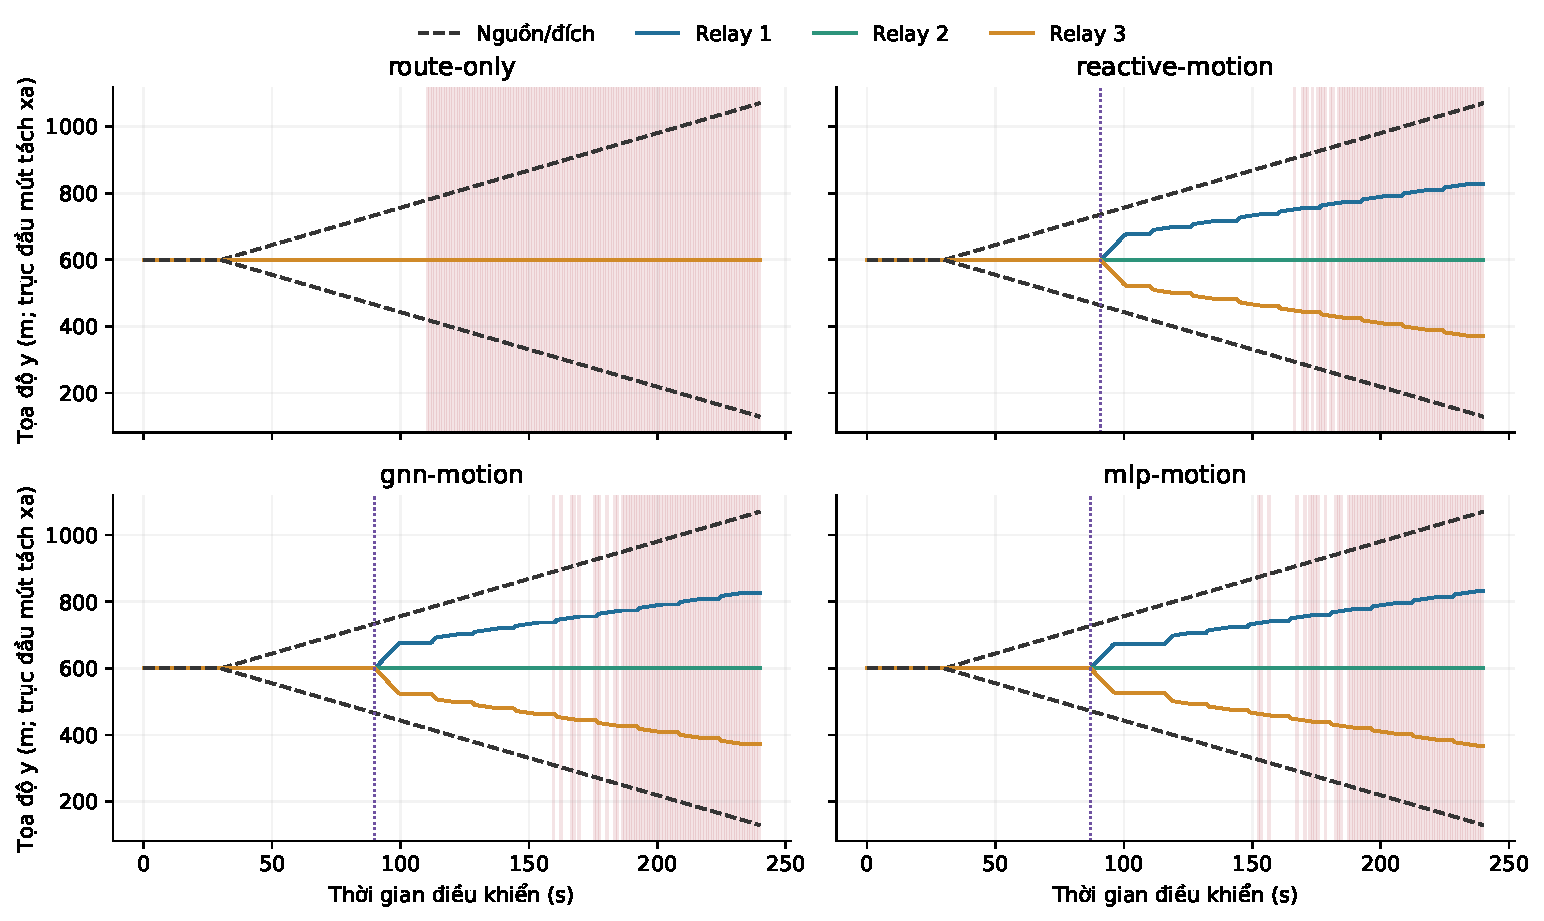
\includegraphics[width=\linewidth]{images/fig_v9_motion_example.pdf}\caption{Ví dụ n5 gradual có layout seed nhỏ nhất, lấy đủ bốn arm; vùng đỏ nhạt là mất kết nối theo probe, đường tím là lần chuyển động đầu tiên. Không chọn seed theo kết quả thuận lợi.}\label{fig:motionexample}\end{figure}

Hình~\ref{fig:motionexample} minh họa hành động thực thi; kết luận lấy từ toàn bộ các khối kịch bản. Số episode có chuyển động trong gradual: \code{gnn-motion}: 40/40; \code{mlp-motion}: 40/40; \code{reactive-motion}: 40/40; \code{route-only}: 0/40.
